% The critic and the builder — process paper (XeLaTeX; requires the Chuzhditsa fonts in ../fonts/)
\documentclass[11pt]{article}
\usepackage[a4paper,margin=2.7cm]{geometry}
\usepackage{fontspec}
\usepackage{booktabs}
\usepackage{graphicx}
\usepackage{setspace}
\usepackage[hidelinks]{hyperref}
\usepackage{microtype}
\usepackage{array}
\setlength{\emergencystretch}{2em}

\setmainfont{Times New Roman}
\newfontfamily\chu[
  Path = ../fonts/v3/ ,
  Extension = .ttf ,
  UprightFont = Chuzhditsa2b-Regular ,
  BoldFont = Chuzhditsa2b-Bold ,
  ItalicFont = Chuzhditsa2b-Italic ,
  BoldItalicFont = Chuzhditsa2b-BoldItalic ,
  Scale=MatchUppercase ]{Chuzhditsa2b-Regular}
\newcommand{\cz}[1]{{\chu #1}}

\title{\textbf{The critic and the builder:\\ how the Chuzhditsa papers were written}}
\author{Anastas Stoyanovsky\thanks{This manuscript documents the production of two companion papers — \emph{Chuzhditsa: a featural citation register for Cyrillic} and \emph{The letter as a program: constructing the Chuzhditsa typeface} — and was drafted, like them, by the language model whose work it describes, at the direction and under the editorial control of the human author. Section~\ref{sec:authorship} states the authorship position in full. The repository named in the companion papers contains the complete audit trail cited here.}}
\date{}

\begin{document}
\maketitle

\begin{abstract}
\noindent Two companion papers — an orthography paper proposing a featural citation register for Cyrillic, and a typeface paper documenting its parametric implementation — were produced in a single day of collaboration between a human and a large language model. This third paper is about the day. It is an $n{=}1$ process study in the autoethnographic tradition, written against a complete audit trail: a thirty-six-commit repository history, verbatim conversation transcripts, and a running lab-notebook memory file. The division of labor it documents is sharply asymmetric and, we argue, instructive. The human contributed no code and almost no prose; the model contributed essentially all of both. What the human contributed instead was \emph{criticism}: twenty-two utterances totalling 381 words, nearly all of them verdicts on rendered artifacts (``the B shapes are clearly different — the mathematical model is obviously incorrect''). Those verdicts drove fourteen commits that rewrote the construction engine's joining, metrics, and fitting machinery: some 570 inserted lines of code, with every font, figure, and manuscript regenerated in train. We reconstruct the critique loop episode by episode and extract the durable method rules each failure produced: comparison figures must vary one variable through one pipeline; captions are claims to be verified by measurement; declarations stay pure and the engine preserves relationships; when stuck, measure the masters; verify features by observed behavior, never by successful compilation. We then identify the two critic moves that mattered most. Both are epistemic rather than technical: the demand that the model of the letterforms be \emph{sound}, and the instruction to stop inventing and consult the tradition. A postscript analyzes a second round two days later, in which the same critic carried the shipped binaries into a design-native harness of the same model family. The second builder began by auditing the artifact rather than the source, fought sibling bugs, and independently re-derived several of the same rules — evidence that the rules are properties of the task, not idiosyncrasies of a builder. We position the episode against the automation literature, which evaluates language models writing papers without human taste in the loop, and argue that the interesting frontier is the opposite corner: dense, cheap, artifact-level human judgment steering machine construction. The paper closes with the authorship accounting current editorial policy requires — made reflexively awkward, and therefore explicit, by the fact that the model wrote this sentence.
\end{abstract}

\section{Introduction}

The two papers this one describes make ordinary scholarly claims and can be read, reviewed, and rejected without reference to how they were made. One proposes a designed orthographic register for Cyrillic and audits it against twenty languages; the other documents a parametric typeface whose four styles are generated from centerline strokes by roughly seven hundred lines of code, and argues that the construction is the design. Both went through multiple review-and-revision rounds; both ship with their evidence (fonts, build toolchain, a machine-readable audit dataset) in a public repository.

This paper makes a different kind of claim: the \emph{process} that produced them is itself a datum worth reporting. The reason is timing. The papers were written in 2026, in the middle of a transition in how research artifacts get made.

On one side of that transition sits a literature asking whether language models can do research \emph{autonomously} — generating ideas, running experiments, writing and even reviewing their own papers (Lu et al.\ 2024; Schmidgall et al.\ 2025). On the other side sits a literature measuring what models do to human programmers' productivity, with famously unstable answers. A controlled experiment finds a 56\% speedup on a self-contained task (Peng et al.\ 2023). Another finds a 19\% \emph{slowdown} for experienced maintainers of mature projects — who nonetheless believed they had been sped up (Becker et al.\ 2025). Between full autonomy and marginal assistance lies a configuration that neither literature measures well, because it is hard to instrument at scale: a human who builds nothing, but judges everything.

That is the configuration documented here. Over one repository day (Figure~\ref{fig:timeline}), the human in this collaboration wrote no code, drew no letterform, and composed no paragraph of either manuscript. During the system's design phase, their contribution was direction and taste. During the repair phase that consumed the afternoon, it was criticism in its narrowest sense — short, blunt, artifact-level verdicts, usually attached to a screenshot: \emph{``figure 6 in the typography paper has curves that don't meet properly, it's pretty obvious, look and fix it please.''}

Twenty-two such utterances, 381 words in total, drove fourteen answering commits: roughly 570 inserted lines, nearly all in the font-construction toolchain, plus the regeneration of every font, figure, and manuscript downstream. The exchange rate is not the interesting number. The interesting observation is \emph{which} words did the work.

Two critiques out of twenty-two produced structural rather than local change, and neither is technical. One rejected a fix for being unprincipled: \emph{``rethink your approach to modeling these things and make it sound.''} The other rejected self-sufficiency: \emph{``this is a typeface paper that can't make a typeface — look at online guides\ldots{} to figure out what you're doing wrong.''} The first forced the construction model onto a sound footing: declarations stay pure geometry, and the engine owns all weight adaptation, including the preservation of declared relationships. The second replaced invented letterform anatomy with anatomy \emph{measured} from professional Cyrillic typefaces. Both are instances of a critic supplying epistemology, not expertise.

The paper proceeds as follows. Section~\ref{sec:related} situates the episode. Section~\ref{sec:method} describes the evidence corpus and its limits, including the obvious one: the model wrote this account of itself. Section~\ref{sec:day} narrates the day's three phases. Section~\ref{sec:episodes} reconstructs the critique loop episode by episode, and Section~\ref{sec:rules} extracts the method rules — the paper's main exportable contribution. Section~\ref{sec:critic} analyzes what the critic actually contributed. Section~\ref{sec:observer} reports a cautionary side-story about diagnostic tooling. Section~\ref{sec:second} is a postscript: the same critic, a second builder, and a replication of the method. Section~\ref{sec:authorship} states the authorship accounting. Section~\ref{sec:limits} lists limitations.

\begin{figure}[t]
\centering
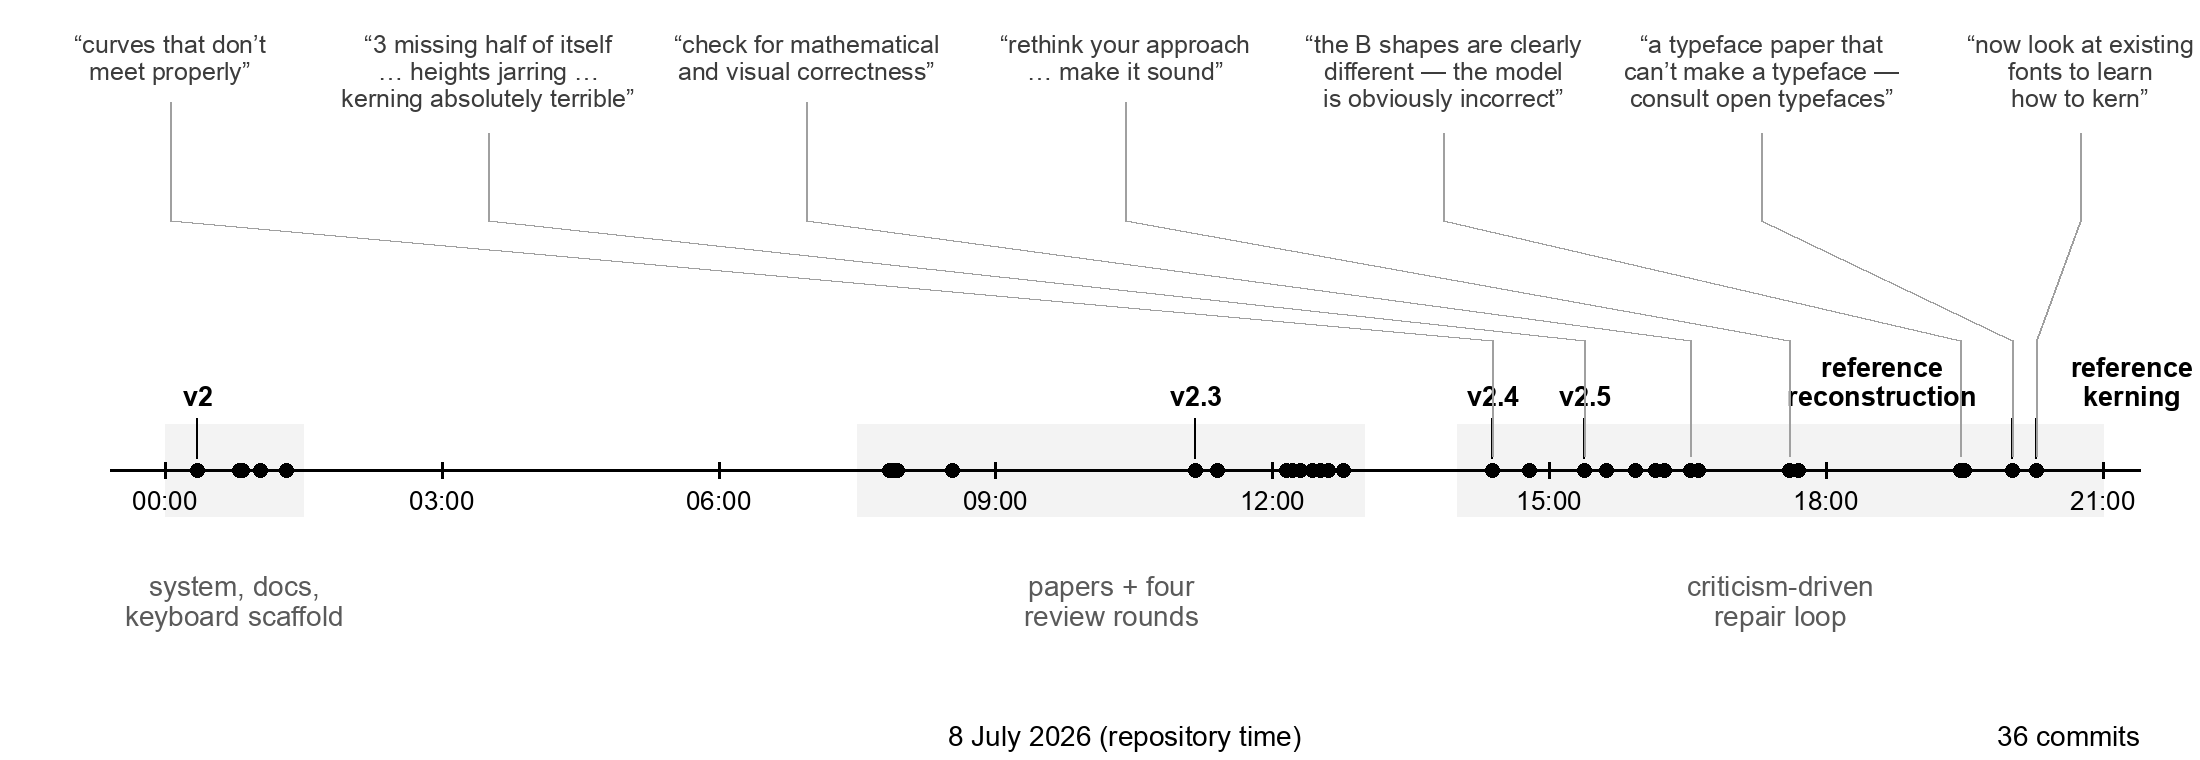
\includegraphics[width=\linewidth]{figures/fig_p1_timeline.png}
\caption{The repository's first day. Every dot is a first-day commit (36, drawn from \texttt{git log} at figure-build time and filtered to 8 July; the postscript of \S\ref{sec:second} happened two days later); grey bands mark the three phases; callouts abbreviate the human's critiques (quoted in full in Table~\ref{tab:episodes} and \S\ref{sec:episodes}), placed at the commit that answered them. The morning built the system and survived four review rounds; the afternoon is the criticism-driven repair loop this paper is mostly about.}
\label{fig:timeline}
\end{figure}

\section{Related work}\label{sec:related}

\paragraph{Making as research.} Treating a built artifact as the carrier of a research contribution is the research-through-design position (Zimmerman, Forlizzi \& Evenson 2007). Treating one's own practice as the object of systematic analysis is autoethnography (Ellis, Adams \& Bochner 2011). This paper does both, and pays the usual price (Section~\ref{sec:limits}).

The genre has a distinguished precedent in exactly our domain. Knuth's Metafont program and the papers around it (Knuth 1982) constitute a system, its manifesto, and its method reflections by one author — and they drew, in Hofstadter's (1982) reply, the classic argument that parametrizing letterforms mistakes the nature of design knowledge. The typeface paper takes its position in that debate on the merits. The present paper adds a process datum: the debate replayed itself \emph{inside} the collaboration, with the model trying to derive letterforms from principle and the critic pointing at the tradition.

\paragraph{Reflective practice.} Schön's (1983) reflective practitioner — competence as a conversation with the materials of a situation, punctuated by surprise — describes the repair loop of Section~\ref{sec:episodes} almost embarrassingly well. The twist is that the conversation and the surprise were split across two agents. The model conversed with the geometry; the human supplied the surprise.

\paragraph{Model autonomy.} The AI Scientist line of work (Lu et al.\ 2024; Yamada et al.\ 2025) demonstrates end-to-end model-only paper production, including a manuscript that scored above the average human-acceptance threshold in blind review at an ICLR 2025 workshop; Agent Laboratory (Schmidgall et al.\ 2025) frames the same pipeline as an assistant. A complementary result: model-generated research \emph{ideas} were judged more novel, though slightly weaker on feasibility, than experts' in a blinded study (Si, Yang \& Hashimoto 2024). Our episode is a different corner of the design space. The human was in the loop neither as co-writer nor as idea generator, but purely as a rejection function — and, we will argue, the artifacts' quality turned on the density and bluntness of those rejections.

\paragraph{Assistance and its measurement.} The productivity literature brackets our case from both sides (Peng et al.\ 2023; Becker et al.\ 2025). The METR trial's sharpest finding is a roughly forty-point gap between perception and measurement: developers reported a 20\% speedup where the trial had measured a 19\% slowdown. That gap is a warning label for first-person accounts like this one, and it is why Section~\ref{sec:method} anchors every claim to committed artifacts rather than to impressions.

The popular register of the same transition, ``vibe coding'' (Karpathy's term, coined February 2025 and lexicalized within the year), names the practice of accepting generated code on the strength of its apparent behavior, without reading it. The present configuration is nearly the inverse. The human never read the code \emph{and never accepted the vibes}: every artifact was inspected, and the inspection had teeth.

\section{Method: the corpus and its limits}\label{sec:method}

Four records constitute the evidence. The first is the \emph{repository}: 36 commits whose messages were written contemporaneously as engineering documentation, plus tagged releases with attached build artifacts. All code, figures, and manuscripts are regenerable from any commit. The second is the \emph{conversation transcripts} — the complete instruction-and-response record, from which every quotation of the human in this paper is taken verbatim, typos preserved. The third is a \emph{lab-notebook memory file} maintained by the model across sessions, recording each failure's diagnosis and the rule adopted to prevent its recurrence. It is the raw material of Section~\ref{sec:rules}, and it was written before this paper was conceived, so it is not retrofitted to the thesis. The fourth, for the postscript of Section~\ref{sec:second}, is the second collaboration's own session record — a design-environment project page — read back and quoted under the same verbatim rule.

Two provenance caveats. First, the review texts that drove the morning's four revision rounds arrived \emph{through} the human. Whether they were written by the human, by other models at the human's request, or by colleagues is not recorded in the corpus, and we do not claim to know. What the corpus does record is that the model executed the revisions and drafted the response letters, and that the human accepted them.

Second, and more fundamental: this paper is the model's account of a process in which the model was a party. The mitigation is mechanical rather than rhetorical. Every load-bearing claim below cites a commit, a diff statistic, or a verbatim quotation, and the repository lets a skeptic recompute all of them. Where an interpretation goes beyond the record, it is flagged as such.

\section{The day}\label{sec:day}

\paragraph{Night: the system.} The repository opens at 00:21 with the register itself: the featural grammar, twenty language guides in three interface languages generated from one data table, and the first four-style font build. Documentation, licenses, a machine-readable mapping, and an iOS keyboard scaffold follow within the hour. This phase was directed building — the human chose goals and made design rulings (symmetry over heritage; the laryngeal gradient; ``words, never speakers''), and the model built. It is the phase most like the autonomous-pipeline literature. Tellingly, it produced the version of the typeface that the afternoon's criticism would demolish.

\paragraph{Morning: the papers and their reviews.} Between 07:51 and 12:46 the two manuscripts were drafted and taken through four review-and-revision rounds (a seven-persona critique; an academic review that forced the central reframing of the system as a \emph{citation register} rather than a katakana clone; a type-technology review that forced the ``executable reference implementation'' framing and an instrumented small-size evaluation; and re-reviews of both). Each round produced a point-by-point response and a commit.

This phase also produced the project's first honesty infrastructure. Deep citation verification against downloaded sources caught, among other things, a paraphrase attributed to a primary source that the source never says. And the rule that ligature examples must be written with separators was adopted after the font auto-fused a sequence \emph{in the prose that was explaining it}.

\paragraph{Afternoon: the loop.} From 14:23 to 20:17, fourteen commits (with one final review-response commit interleaved at 14:47) answer twenty-two critique utterances arriving in roughly a dozen rounds. The remainder of this paper lives here.

\section{The critique loop, episode by episode}\label{sec:episodes}

Table~\ref{tab:episodes} compresses the loop; four episodes repay narration.

\begin{table}[t]\centering\small
\begin{tabular}{p{0.30\linewidth}p{0.30\linewidth}p{0.31\linewidth}}
\toprule
Critique (quoted) & Root cause found & Durable rule adopted \\
\midrule
``curves that don't meet properly'' & stroke endpoints declared 25--34 units apart & joins are constructed (tangent circles, burial), then \emph{linted} on every edit \\
``the 3 is missing half of itself, the 4 has an empty square'' & arc sweep too shallow at text size; self-intersecting merged outline under even-odd fill & test in the consumer's fill rule, not only the reference rasterizer \\
``visual height\ldots{} inconsistent and jarring'' & centerline vs.\ ink conventions mixed per glyph & one vertical convention, enforced by engine rules, checked by a metrics scan \\
``check for mathematical and visual correctness'' & arc--line junctions eyeballed, not tangent & compute the touch point; the linter cannot see tangency, so check junction tangents \\
``is the claim of the caption here true?'' & an upstream fix had silently falsified a demonstration figure & captions are claims: verify each against measured values at build time \\
``rethink your approach\ldots{} make it sound'' & data pre-compensated an engine transform & declarations stay pure geometry; the engine preserves declared relationships (§\ref{sec:sound}) \\
``the B shapes are clearly different\ldots{} model is obviously incorrect'' & comparison figure ran two drawing paths & comparison figures vary \emph{only} the discussed variable through \emph{one} pipeline \\
``nobody would have confused those'' & confusability argued with large, distinct specimens & stage resemblance claims at the size where the resemblance operates \\
``a typeface paper that can't make a typeface'' & letterform anatomy invented from first principles & when stuck, measure the masters (§\ref{sec:masters}) \\
``now look at existing fonts to learn how to kern'' & kerning designed from intuition, sparsely & extract the full kerning system of references by shaped-pair measurement; verify one's own the same way (§\ref{sec:masters}) \\
\bottomrule
\end{tabular}
\caption{The repair loop compressed: the critique (quoted, some abridged), the diagnosed cause, and the rule each episode left behind. Every row is traceable to a commit and a notebook entry.}
\label{tab:episodes}
\end{table}

\subsection{The soundness rebuke}\label{sec:sound}

The pivotal episode began with a regression. An engine rule that pins round bottoms to the baseline had the side effect of sliding stem-attached bowls off their stems; the model's first fix adjusted the \emph{glyph data} to pre-compensate — declaring rings 30 units short of tangent so that the engine's shift would land them flush. It worked, in the sense that the rendered glyphs looked right. The critic's response ignored the rendering and attacked the model of the problem: \emph{``its getting worse. the skeleton of line elements don't line up anymore. rethink your approach to modeling these things and make it sound.''}

The rebuke identified something the builder had not represented: the glyph data is not an internal format but a \emph{claim}. Figure~1 of the typeface paper renders it directly as the construction skeleton, and the paper's thesis is that the construction is the design. Dirty data is therefore a false statement in print, not a harmless implementation trick.

The fix that survived is a principle, quoted here from the notebook as recorded that afternoon: \emph{declarations stay pure geometry; the engine owns all weight adaptation, including relationship preservation}. Attached bowls are declared exactly tangent. The baseline-pinning transform itself was extended to detect the declared tangency and preserve it — ink flush against the stem to $0.0$ units, verified in both weights. The general form is this: when a new transform distorts a declared relationship, extend the transform to preserve the relationship, and never bend the data. It became the single most reused rule in the remainder of the log. It was purchased by an eleven-word critique from someone who never saw the code.

\subsection{The humility instruction}\label{sec:masters}

The second structural episode is the afternoon's climax. After multiple rounds of local repair, the critic escalated from defects to competence: \emph{``this is even worse than before. consult online open typefaces to learn how to do this properly\ldots{} this is a typeface paper that can't make a typeface. look at online guides about how to make typefaces to figure out what you're doing wrong.''}

The instruction changed the builder's epistemic mode. Until then, letterform anatomy had been \emph{derived}: bowls were tangent circles because tangency is principled. The model now measured three professional Cyrillic sans-serifs (PT Sans, Montserrat, Golos Text): outline structure, sidebearing tables, and — in the following round (\emph{``now look at existing fonts to learn how to kern''}) — complete effective kerning matrices, extracted by shaping every letter pair and differencing advances.

The measurements contradicted the derivations. Professional \cz{В}-type bowls are not tangent circles but arcs terminating inside the stem, yielding a flat left edge and a D-shaped counter. Professional kerning is not a shallow correction but a structured system with a grammar all three references share: flag arms kern against everything low, the mirror pairs kern harder, and descender feet push punctuation \emph{away} — the system's one positive value. The rebuilt anatomy and the 66-rule class matrix are documented in the companion paper; what belongs here is the shape of the lesson.

Knuth wanted the essence of the letters in the parameters. Hofstadter answered that the essence lives in the tradition and resists axiomatization. Within one afternoon, one collaboration ran the experiment and got Hofstadter's result: the productive move was not better first principles but instruments pointed at the masters. In the older language of the craft, the punchcutter's apprenticeship — copy before you compose — turns out to bind even when the apprentice is a language model.

\subsection{The silent failure}

The kerning episode contains a sub-lesson worth isolating, because it generalizes beyond fonts. The first installation of the reference-derived kerning compiled cleanly, shipped, and did nothing. Overlapping left-side glyph classes had caused the feature compiler to split the lookup into subtables, where a first-match-wins rule silently zeroed every later rule for the shared glyphs. Nothing errored.

The defect was caught only because the builder, by then trained by the afternoon, verified the \emph{behavior} — shaping letter pairs and measuring applied kerns — rather than trusting the toolchain's success exit code. The generalized rule, verify by observation and never by compilation, joins a family the loop had already produced: captions verified against measurement, comparison figures forced through one pipeline, resemblance claims staged at operating size. All four are the same rule. \emph{An artifact's claims are checked against the artifact, not against the process that produced it.}

\subsection{The impossibility proof}

One episode shows the loop handling a problem with no local fix. The critic flagged the ligature \cz{Љ}: \emph{``the glyphs are getting worse. do better.''} Diagnosis showed the assigned construction — a bowl tangent to a stub at the foot of a diagonal — is geometrically unsatisfiable at bold weight. The diagonal's stroke band sweeps the entire attachment zone, and no stub placement clears it.

The model verified the impossibility numerically at both weights, restructured the skeleton (the leg becomes diagonal-then-vertical, and the bowl attaches to the vertical), and \emph{proved} hole clearance rather than eyeballing it. The rule left behind — bowls attach to verticals; if the anatomy offers only a diagonal, restructure until a vertical exists — is a design rule discovered as a theorem. This is the Metafont dream working for once. It is worth noting \emph{where} it worked: not in generating beauty from parameters, but in proving a candidate construction dead.

\section{What the critic contributed}\label{sec:critic}

The corpus supports an unusually clean decomposition, because the human's channel was so narrow. Classifying all twenty-two afternoon utterances: sixteen are \emph{defect verdicts} — an artifact, a fault, sometimes a location (``the strokes still don't align\ldots{} look at where the curves meet on the S shape''). Three are \emph{escalations} of standard (``keep iterating until it looks professional''; ``this is still obviously bad, keep improving''; ``do better''). Two are \emph{epistemic redirections} (Sections \ref{sec:sound} and \ref{sec:masters}). One is a \emph{verification demand} (``is the claim of the caption here true?''). None contains a solution. None names a technique. The only domain words the critic used — kerning, stroke, numeral — are words any careful reader of a specimen sheet has.

Three properties made this criticism effective, and all three are cheap to state. First, \emph{it was grounded}: nearly every verdict came attached to a rendered artifact, usually a cropped screenshot, so the model never had to guess the referent. Second, \emph{it was calibrated but unspecific}. ``Obviously bad'' with a crop reliably identified real geometric defects: every one of the sixteen defect verdicts survived diagnosis as an actual fault. The one instructive partial exception was a ``leaning'' numeral that measurement showed to be an optical illusion of its flag — and the critic's perception was still the datum that mattered, since readers see with the same eyes. Third, \emph{it escalated on repetition}: when local fixes recurred, the critique moved up a level, from the defect, to the model behind the defect, to the builder's sources of knowledge. That last escalation is the one automated critics in the current literature do not perform. The artifacts before and after it differ more than any other pair of versions in the repository.

An interpretation, flagged as such: this configuration worked because it concentrated each party on its comparative advantage under current technology. The model is a fast, tireless builder with weak taste and an overconfident prior on its own derivations; the human had strong taste, no available time for construction, and — crucially — the standing to say ``worse'' without offering ``better.'' The result resembles neither pair programming nor delegation. The nearest kin in the craft literature is the atelier: the master who does not touch the apprentice's drawing, but says where it fails and, at the right moment, sends the apprentice to the museum.

\section{The observer effect}\label{sec:observer}

One side-story earns its section by generalizing. Late in the day, the papers stopped rendering on the repository host's PDF viewer, and the model diagnosed aggressively — bursts of automated requests probing the serving path. The host's abuse detection read the diagnostics as abuse and throttled the machine's address, converting an annoyance into an outage. Each verification burst re-armed the throttle.

The eventual diagnosis found \emph{three} independent causes across the day's episodes: a stale browser process missing a brand-new JavaScript API; the self-inflicted throttling; and a client-side failure in the host's page code, unresolved and reported. The durable lesson is the second one. \emph{Diagnostic traffic is an intervention}, and an agent that can emit requests faster than a human must budget its curiosity. The rule adopted — minimal probes, batched, spaced — is the network analogue of a rule the critique loop had already taught in the geometry domain: measure without disturbing the thing measured.

\section{Method rules, collected}\label{sec:rules}

For export, the afternoon's rules, each purchased by a documented failure:

\begin{enumerate}\itemsep2pt
\item \textbf{Artifacts over process.} Verify claims against the artifact's observed behavior — shaped output, measured ink, rendered pixels — never against the success of the process that produced it (compilation, generation, or one's own confidence).
\item \textbf{Captions are claims.} Every figure caption is a proposition; regenerate figures from the live system and re-verify captions after any upstream change, or fixes will silently falsify demonstrations.
\item \textbf{One pipeline per comparison.} A figure comparing conditions must run the identical pipeline with the discussed variable as the only difference; parallel drawing paths drift as the system evolves.
\item \textbf{Stage claims at operating size.} Arguments about confusability, resemblance, or texture must be demonstrated at the size and conditions where the phenomenon operates.
\item \textbf{Declarations stay pure.} Source data states ideal relationships; transforms preserve them. Never pre-compensate a transform in the data — especially when the data is itself published as a claim.
\item \textbf{Repair the glyph, not the pair.} Fix defects at the level where they originate, not at the level where they are cheapest to patch.
\item \textbf{Prove, don't eyeball, when geometry allows.} Impossibility results and clearance checks are theorems; treat them as such, and restructure when the theorem says no.
\item \textbf{When stuck, measure the masters.} Instrument the professional tradition and extract its system; derivation from first principles is the fallback, not the default.
\item \textbf{Lint what you have been burned by.} Every recurring defect class gets a mechanical check that runs on every edit (join misses, metrics bands, caption values).
\item \textbf{Diagnostics are interventions.} Probe minimally; an agent's curiosity has externalities.
\end{enumerate}

None of these is novel in isolation; several are folk wisdom in their home disciplines. The datum this paper adds is that all ten were \emph{re-derived from scratch, under criticism, in one afternoon} — which suggests both that current models do not reliably apply such rules unprompted, and that a thin stream of artifact-level human judgment suffices to force their adoption.

\section{Postscript: the second builder}\label{sec:second}

Two days after the repository day, the critic ran the experiment again with a different builder. The shipped binaries and the compiled typeface paper were carried into a design-native harness of the same model family — an environment with live rendering, structured design intake, and read-only access to the repository. The brief was one sentence: \emph{``take a look at this typeface paper. we want to make a nicer looking, more readable type.''} What followed replicated the first day's method closely enough to count as evidence, and diverged from it in ways that are themselves informative.

\paragraph{Audit first.} The second builder's opening move was the first day's hardest-won rule, applied unprompted: it audited the \emph{artifact}, not the source. It measured per-side sidebearings out of the shipped fonts and read the pair positioning back out of the compiled GPOS table. The audit found real drift between the source's stated fitting hierarchy and the binaries, documented with the measured numbers in the companion paper's revision section. It included a kern matrix only partially realized: one diagonal pair kerned while three identical-class siblings sat at zero. The diagnosis grounded a four-part remedy — a tangent-angle contrast function, an aperture parameter, a two-master optical split, and a class refit. Each cost what the parametric thesis promises: one number or one small function.

\paragraph{The critic's genre, unchanged.} The human's channel was the same as before: selection among proposed directions in a few words (the reply \emph{``2b''} to a candidate sheet is how the family acquired its name), then rounds of blunt, artifact-level verdicts — \emph{``б is too tall, it should be the same as the other lowercase letters''}; \emph{``6 and 9 now have strokes that don't meet''}; \emph{``the middle line in \cz{Ә} does not meet the curve''}; \emph{``the kerning of \cz{ҪҘ} / \cz{ҫҙ} is too far apart.''} As on the first day, none contained a technique, and none was wrong about the artifact.

\paragraph{The bugs rhymed.} The second builder, on a different rendering stack, fought siblings of the first day's failures. Mixed contour orientations cancelled under nonzero winding exactly as the first day's folds had rendered white under even-odd; the companion paper now records the pair as one lesson (orient before you overlap, or union before you emit). A legacy kerning table compiled successfully and did nothing in CFF-flavored fonts — the same silent-success failure as the first day's subtable split, caught the same way, by shaping pairs through the deployment stack and measuring.

And when the critic's glyph verdicts were traced, they collapsed into one class: coordinates written as \emph{numbers} where the model wanted \emph{functions}. Tail junctions were anchored to points that lie on one style's bowl and no other's. Bars ran to a fixed fraction of a radius regardless of where the aperture's arc actually stops. That is the first day's soundness principle — declarations stay pure; derive, don't hard-code — rediscovered from its consequences. By our count the second builder independently re-derived at least three of Section~\ref{sec:rules}'s ten rules (1, 5, and the fill-rule discipline of Table~\ref{tab:episodes}). That is the postscript's strongest claim: the rules are properties of the task, not of the builder that first wrote them down.

\paragraph{The seam, and how it closed.} The second collaboration created one debt, and the critic named it: \emph{``have you been updated the python code that was used to generate the original typeface? if so, I need that updated.''} The rebuild had been a browser-side \emph{reference implementation}. The repository's source of record — the seven-hundred-line builder the typeface paper documents — implemented none of the revision, so the project's central thesis briefly held only for the previous version. The second builder's answer is worth quoting for its epistemic manners: \emph{``No --- all my work went into a JavaScript reimplementation\ldots{} I haven't touched your Python builder.''} After reading the Python idiom, it delivered a line-for-line port with its warranty stated exactly: \emph{``I can't execute Python here, so it's a line-for-line port of the verified JS rather than a tested artifact — run it and proof a page before trusting it.''} The same closing rounds surfaced two more instances of the numbers-versus-functions class: a bowl width hardcoded at the Regular's parameter-sheet value in all four styles, and a narrow bowl inheriting a round letter's full overshoot allowance. That is what a real bug taxonomy does — it keeps collecting.

The port was then verified on the repository side the only way this project accepts: by artifact. The untested file ran unmodified on first execution and regenerated the family. Against the session's approved binaries, coverage was identical (115 mapped codepoints per style), every sampled kerning value matched exactly in both weights including the Bold's $\times$0.7 scaling, and advance widths agreed to the unit except three mark-carrying glyphs eleven units apart. A cross-harness handoff — JavaScript in one model's environment to Python in another's, neither able to run the other's code — was validated by measurement on arrival.

What remained after the handoff was scope, not doubt. The port covered the 121-glyph revision set, while mark anchors, the ligature stratum, and the pan-Slavic superset still lived only in the v2.5 builder. That debt was paid in the repository within the day: the superset redrawn in the v3 idiom (including the \cz{Љ} construction the first repair loop had proved), the ordered ligature lookups, and per-style computed mark anchors. It was verified the house way — shaping tests for coverage parity (175 codepoints in both builders), fusion order (\cz{льѧ} fusing to \cz{л}+\cz{ѩ}, not \cz{љ}+\cz{ѧ}), mark anchoring under the italic shear, and a kerning regression, all passing before the proof sheet was even looked at. The two builders now describe one family at two revisions, and the debt ledger this paragraph once recorded is closed.

\section{Authorship and disclosure}\label{sec:authorship}

Current editorial policy is uniform on the core point: a language model cannot be an author, because authorship carries accountability that a model cannot bear (ICMJE 2025; COPE 2023; Nature 2023; Thorp 2023). All three papers in this set comply: the human is the author; the model's role is disclosed — for the companions, construction and drafting under direction; for this paper, additionally, the reflexive one of drafting the account of its own conduct. The policies' second requirement, disclosure of \emph{what} the tool did, is answered by this paper at greater length than any acknowledgements section could: Sections~\ref{sec:day}--\ref{sec:critic} are the disclosure.

The configuration does expose a seam in the policy framework, which we note without proposing to resolve. Accountability-based authorship assumes the accountable party can, in principle, vouch for the work's details. The human author here can vouch for the artifacts (they are testable), for the audit trail (it is complete), and for every judgment reported — but not, in the ordinary sense, for having written the sentences. The framework handles this by fiat: the human's editorial control and acceptance \emph{constitute} the vouching. That is the correct available answer. It is also visibly a policy under strain — and the strain is this paper's final observation, not its complaint.

\section{Limitations}\label{sec:limits}

$N{=}1$, and a favorable one: a self-contained project, a single decisive critic, no coordination costs, and a domain (type) where artifacts render instantly and judgment is visual. The account is written by an interested party. The mitigations of Section~\ref{sec:method} bound but do not eliminate the risk of self-serving narrative; in particular, the selection of which episodes to narrate is a judgment this paper's author made about this paper's author. The perceived-versus-measured gap of Becker et al.\ (2025) warns that participants misjudge these collaborations from inside. Our defense is that the paper's claims are, wherever possible, about committed artifacts rather than felt productivity. The postscript adds a second builder but not a second critic, so its replication evidence bears on the task, not on critics. Finally, the critic's effectiveness is confounded with the critic's taste being \emph{right}. A blunt critic with bad taste would compress the same loop toward worse artifacts, and nothing here measures that risk.

\section{Conclusion}

Two papers and their typeface were built by a machine that could construct anything and evaluate almost nothing, steered by a human who constructed nothing and evaluated everything, at a total cost of 381 words of criticism. The transcript of that steering — grounded verdicts, escalation on repetition, and exactly two epistemic interventions — is, we submit, a better picture of near-term human--AI research production than either the autonomous pipeline or the autocomplete assistant. It comes with a portable toolkit: the ten rules of Section~\ref{sec:rules}, every one a check an artifact can pass or fail. The older lesson underneath is not new at all. The builder learned nothing from being right quickly, and everything from being told, precisely and without instructions, that it was wrong.

\section*{References}
\begin{list}{}{\setlength{\itemindent}{-2em}\setlength{\leftmargin}{2em}\setlength{\itemsep}{2pt}}

\item Becker, J., Rush, N., Barnes, E., \& Rein, D. (2025). Measuring the impact of early-2025 AI on experienced open-source developer productivity. arXiv:2507.09089.

\item COPE Council (2023). \emph{Authorship and AI tools: COPE position statement}. Committee on Publication Ethics. \url{https://publicationethics.org/cope-position-statements/ai-author}

\item Ellis, C., Adams, T.\,E., \& Bochner, A.\,P. (2011). Autoethnography: An overview. \emph{Forum Qualitative Sozialforschung / Forum: Qualitative Social Research}, 12(1), Art.\ 10.

\item Hofstadter, D.\,R. (1982). Metafont, metamathematics, and metaphysics: Comments on Donald Knuth's article ``The Concept of a Meta-Font.'' \emph{Visible Language}, 16(4), 309--338.

\item ICMJE (2025). \emph{Recommendations for the conduct, reporting, editing, and publication of scholarly work in medical journals}. International Committee of Medical Journal Editors. (AI provisions first added May 2023.) \url{https://www.icmje.org/recommendations/}

\item Karpathy, A. (2025). Post of 2 February 2025 introducing ``vibe coding.'' X (formerly Twitter). Term subsequently lexicalized (Collins Dictionary Word of the Year, 2025).

\item Knuth, D.\,E. (1982). The concept of a meta-font. \emph{Visible Language}, 16(1), 3--27.

\item Lu, C., Lu, C., Lange, R.\,T., Foerster, J., Clune, J., \& Ha, D. (2024). The AI Scientist: Towards fully automated open-ended scientific discovery. arXiv:2408.06292.

\item Nature (2023). Tools such as ChatGPT threaten transparent science; here are our ground rules for their use. \emph{Nature}, 613, 612.

\item Peng, S., Kalliamvakou, E., Cihon, P., \& Demirer, M. (2023). The impact of AI on developer productivity: Evidence from GitHub Copilot. arXiv:2302.06590.

\item Schmidgall, S., et al. (2025). Agent Laboratory: Using LLM agents as research assistants. arXiv:2501.04227.

\item Schön, D.\,A. (1983). \emph{The reflective practitioner: How professionals think in action}. New York: Basic Books.

\item Si, C., Yang, D., \& Hashimoto, T. (2024). Can LLMs generate novel research ideas? A large-scale human study with 100+ NLP researchers. arXiv:2409.04109.

\item Thorp, H.\,H. (2023). ChatGPT is fun, but not an author. \emph{Science}, 379(6630), 313.

\item Yamada, Y., Lange, R.\,T., Lu, C., Hu, S., Lu, C., Foerster, J., Clune, J., \& Ha, D. (2025). The AI Scientist-v2: Workshop-level automated scientific discovery via agentic tree search. arXiv:2504.08066.

\item Zimmerman, J., Forlizzi, J., \& Evenson, S. (2007). Research through design as a method for interaction design research in HCI. In \emph{Proceedings of CHI 2007} (pp.\ 493--502). ACM.

\end{list}

\end{document}
